% !TeX program = xelatex
% !TeX encoding = utf-8
\documentclass[aspectratio=169, 11pt]{beamer}

% ==============================================================================
% Cấu hình font và ngôn ngữ
% ==============================================================================
\usepackage{fontspec}
\defaultfontfeatures{Ligatures=TeX}
\setsansfont{Segoe UI}[
  BoldFont = {Segoe UI Bold},
  ItalicFont = {Segoe UI Italic},
  BoldItalicFont = {Segoe UI Bold Italic}
]
\setmonofont[Scale=0.90]{Consolas}[
  BoldFont = {Consolas Bold},
  ItalicFont = {Consolas Italic},
  BoldItalicFont = {Consolas Bold Italic}
]

\usepackage{amsmath,amssymb}
\usepackage{booktabs}
\usepackage{array}
\usepackage{graphicx}
\usepackage{xcolor}
\usepackage{fancyvrb}
\usepackage[many]{tcolorbox}
\usepackage{tikz}
\usetikzlibrary{arrows.meta, positioning, calc, patterns, shapes.geometric}

\graphicspath{{../assets/images/}{../assets/images/figures/}{./}{figures/}}

% ==============================================================================
% Bảng màu giao diện tối giản (Chuẩn Đen - Xám Bách Khoa)
% ==============================================================================
\definecolor{DarkMain}{RGB}{20, 20, 20}       % Màu chủ đạo
\definecolor{BoxMain}{RGB}{222, 225, 230}    % Màu khối chính
\definecolor{BoxDeep}{RGB}{185, 189, 196}    % Màu gợn sóng
\definecolor{BoxSub}{RGB}{246, 247, 249}     % Màu khối phụ
\definecolor{DisabledBg}{RGB}{236, 237, 240} % Màu trạng thái vô hiệu hóa
\definecolor{CodeBg}{RGB}{247, 248, 250}     % Màu nền khối mã nguồn
\definecolor{TextDark}{RGB}{20, 20, 20}      % Màu chữ chính
\definecolor{TextMuted}{RGB}{100, 102, 108}  % Màu chữ chú thích

% ==============================================================================
% Cấu hình giao diện Beamer
% ==============================================================================
\useinnertheme{default}
\useoutertheme{default}
\setbeamertemplate{navigation symbols}{}
\setbeamersize{text margin left=0.95cm, text margin right=0.95cm}

\setbeamercolor{background canvas}{bg=white}
\setbeamercolor{normal text}{fg=TextDark}
\setbeamercolor{frametitle}{fg=DarkMain, bg=white}
\setbeamercolor{itemize item}{fg=DarkMain}
\setbeamercolor{itemize subitem}{fg=DarkMain}
\setbeamercolor{enumerate item}{fg=DarkMain}

% Định dạng danh sách
\setbeamertemplate{itemize item}{\textbf{\color{DarkMain}--}}
\setbeamertemplate{itemize subitem}{\textbf{\color{TextMuted}--}}
\setbeamertemplate{enumerate item}{\textbf{\color{DarkMain}\insertenumlabel.}}

% Định dạng tiêu đề slide
\setbeamertemplate{frametitle}{
  \vspace{0.30cm}
  \noindent{\fontsize{18pt}{22pt}\selectfont\bfseries\color{DarkMain}\insertframetitle}\par
  \vspace{0.14cm}
  \noindent{\color{DarkMain}\rule{\textwidth}{1.05pt}}\par
  \vspace{0.06cm}
}

% Định dạng chân trang
\newcommand{\currentsectionname}{}
\newcommand{\setsectionfooter}[1]{\renewcommand{\currentsectionname}{#1}}

\setbeamertemplate{footline}{
  \hbox to \paperwidth{%
    \hspace*{0.95cm}%
    {\fontsize{8.2pt}{10pt}\selectfont\color{TextMuted}%
      Chia sẻ trạng thái giữa các widget%
      \ifx\currentsectionname\empty\else\ \textbar\ \currentsectionname\fi
    }%
    \hfill
    {\fontsize{8.5pt}{10pt}\selectfont\bfseries\color{DarkMain}\insertframenumber\,/\,\inserttotalframenumber}%
    \hspace*{0.95cm}%
  }%
  \vspace*{0.26cm}%
}

% ==============================================================================
% Định dạng khối mã nguồn và hình minh họa
% ==============================================================================
\newcommand{\code}[1]{\leavevmode{\ttfamily\color{DarkMain}#1}}
\newcommand{\cmt}[1]{\leavevmode{\itshape\color{TextMuted}#1}}
\newcommand{\hl}[1]{\leavevmode{\bfseries\color{DarkMain}#1}}

\newtcolorbox{codepanel}[1][]{
  enhanced,
  frame hidden,
  borderline west={2.3pt}{0pt}{DarkMain},
  colback=CodeBg,
  sharp corners,
  halign=left,
  left=7pt,
  right=7pt,
  top=4pt,
  bottom=4pt,
  boxsep=0pt,
  before skip=1.5pt,
  after skip=1.5pt,
  #1
}

% Cấu hình sơ đồ TikZ
\tikzset{
  >=Stealth,
  diagbox/.style={
    rectangle,
    rounded corners=2.2pt,
    draw=DarkMain,
    line width=0.9pt,
    fill=BoxMain,
    minimum height=0.90cm,
    align=center,
    font=\small\bfseries,
    text=TextDark
  },
  subbox/.style={
    rectangle,
    rounded corners=2.2pt,
    draw=DarkMain,
    line width=0.9pt,
    fill=BoxSub,
    minimum height=0.90cm,
    align=center,
    font=\small,
    text=TextDark
  },
  ghostbox/.style={
    rectangle,
    rounded corners=2.2pt,
    draw=DarkMain,
    solid,
    line width=0.9pt,
    fill=DisabledBg,
    minimum height=0.90cm,
    align=center,
    font=\small,
    text=TextDark
  },
  flowarrow/.style={
    -{Stealth[length=2.3mm, width=1.7mm]},
    draw=DarkMain,
    line width=0.95pt,
    shorten >= 3pt,
    shorten <= 3pt
  },
  dasharrow/.style={
    -{Stealth[length=2.3mm, width=1.7mm]},
    draw=DarkMain,
    dashed,
    line width=0.9pt,
    shorten >= 3pt,
    shorten <= 3pt
  }
}

\begin{document}

% ==============================================================================
% Slide 1: Trang bìa
% ==============================================================================

% ==============================================================================
% Slide 1: Trang bìa
% ==============================================================================
\begin{frame}[plain]
  \vspace{0.2cm}
  \begin{columns}[c, onlytextwidth]
    \begin{column}{0.13\textwidth}
      \centering
      
\includegraphics[height=1.50cm]{figures/logo_truong.png}
    \end{column}
    \begin{column}{0.72\textwidth}
      \centering
      {\normalsize \textbf{TRƯỜNG ĐẠI HỌC BÁCH KHOA}}\\[0.05cm]
      {\normalsize \textbf{ĐẠI HỌC ĐÀ NẴNG}}\\[0.10cm]
      {\normalsize \textbf{KHOA ĐIỆN TỬ VÀ TRÍ TUỆ NHÂN TẠO}}
    \end{column}
    \begin{column}{0.13\textwidth}
      \centering
      
\includegraphics[height=1.55cm]{figures/logo_khoa.jpg}
    \end{column}
  \end{columns}

  \vspace{0.35cm}
  \begin{center}
    {\normalsize \textit{Báo cáo Tuần 13 - Học phần: Lập trình Đa nền tảng}}
  \end{center}

  \vspace{0.25cm}
  \begin{center}
    {\LARGE \textbf{Chủ đề 11: Chia sẻ trạng thái giữa các widget}}
  \end{center}

  \vspace{0.35cm}
  \begin{center}
    \begin{tabular}{rl}
      \textbf{Giảng viên hướng dẫn:} & TS. Nguyễn Duy Nhật Viễn \\[0.12cm]
      \textbf{Sinh viên thực hiện:}   & Lê Anh Khoa (MSSV: 106230016) \\
                                     & Ngô Quang Thế (MSSV: 106230028) \\[0.12cm]
      \textbf{Lớp sinh hoạt:}        & 23KTMT1
    \end{tabular}
  \end{center}

  \vfill
  \begin{center}
    {\footnotesize \color{TextMuted} Đà Nẵng, 2026}
  \end{center}
  \vspace{0.15cm}
\end{frame}

% ==============================================================================
% Slide 2: Nội dung báo cáo
% ==============================================================================
\setsectionfooter{}
\begin{frame}{Nội dung báo cáo}
  \vspace{-0.15cm}
  \begin{tcolorbox}[
    enhanced,
    colback=CodeBg,
    colframe=DarkMain,
    arc=3pt,
    left=12pt, right=12pt, top=6pt, bottom=6pt
  ]
    \fontsize{9.2pt}{13.2pt}\selectfont
    \begin{enumerate}\setlength{\itemsep}{0.12cm}
      \item \textbf{Phân loại trạng thái và nguyên tắc sở hữu}\newline
            {\footnotesize\color{TextMuted}Phân biệt Ephemeral vs App State; Single Source of Truth; quy tắc đặt state tại LCA.}
      \item \textbf{Truyền dữ liệu và vấn đề Prop Drilling}\newline
            {\footnotesize\color{TextMuted}Cơ chế Constructor/Callback; phân tích code nhận truyền tiếp và hiện tượng build lan truyền.}
      \item \textbf{Các cơ chế chia sẻ trạng thái trong Flutter}\newline
            {\footnotesize\color{TextMuted}Cấu trúc InheritedWidget tra cứu trực tiếp; đặc tính của ValueNotifier và ChangeNotifier.}
      \item \textbf{Thực nghiệm: Ứng dụng TaskFlow \& So sánh thực tế}\newline
            {\footnotesize\color{TextMuted}Đo lường số lần build giữa 2 trường hợp, so sánh và chọn cách dùng phù hợp.}
    \end{enumerate}
  \end{tcolorbox}
\end{frame}

% ==============================================================================
% Slide 3: Phân công công việc
% ==============================================================================
\begin{frame}{Phân công công việc}
  \vspace{0.25cm}
  \renewcommand{\arraystretch}{1.55}
  \setlength{\tabcolsep}{2.6pt}
  \begin{tabular}{@{} c >{\raggedright\arraybackslash}p{2.75cm} >{\raggedright\arraybackslash}p{5.55cm} >{\centering\arraybackslash}p{2.45cm} c @{}}
    \toprule[0.9pt]
    {\bfseries\color{DarkMain}STT} &
    \multicolumn{1}{l}{{\bfseries\color{DarkMain}Họ và tên}} &
    \multicolumn{1}{l}{{\bfseries\color{DarkMain}Nội dung đảm nhiệm}} &
    \multicolumn{1}{c}{{\bfseries\color{DarkMain}Slide}} &
    {\bfseries\color{DarkMain}Đóng góp} \\
    \midrule[0.5pt]
    01 & Ngô Quang Thế\newline{\footnotesize\color{TextMuted}106230028} &
    Phân loại trạng thái, Nguyên tắc LCA, Vấn đề Prop Drilling, Cơ chế InheritedWidget, ChangeNotifier, ValueNotifier &
    1--11 & 50\% \\[0.18cm]
    02 & Lê Anh Khoa\newline{\footnotesize\color{TextMuted}106230016} &
    Ứng dụng TaskFlow, Thực nghiệm Trường hợp 1 \& 2, Đo lường số lần build, Cải tiến ValueNotifier \& Kết luận &
    12--21 & 50\% \\
    \bottomrule[0.9pt]
  \end{tabular}
\end{frame}

% ==============================================================================
% Slide 4: Hai loại trạng thái: Ephemeral và App State
% ==============================================================================
\setsectionfooter{Cơ sở lý thuyết}
\begin{frame}{Hai loại trạng thái: Ephemeral và App State}
  \vspace{0.18cm}
  \begin{columns}[c, onlytextwidth]
    \begin{column}{0.48\textwidth}
      \centering
      \begin{tikzpicture}
        \node[subbox, text width=4.5cm, align=center, minimum height=1.15cm] (eph) at (0, 0)
          {\textbf{Ephemeral State (Cục bộ)}\\[-1pt]{\scriptsize\normalfont\color{TextMuted}Tạm thời trong 1 widget (Tab, Expansion, Form)}};
      \end{tikzpicture}
    \end{column}
    \hfill
    \begin{column}{0.48\textwidth}
      \centering
      \begin{tikzpicture}
        \node[diagbox, text width=4.5cm, align=center, minimum height=1.15cm] (app) at (0, 0)
          {\textbf{App State (Chia sẻ)}\\[-1pt]{\scriptsize\normalfont\color{DarkMain}Dùng chung nhiều nơi (Danh sách việc, Tiến độ, Phân bổ)}};
      \end{tikzpicture}
    \end{column}
  \end{columns}

  \vspace{0.35cm}
  \begin{itemize}\setlength{\itemsep}{0.22cm}
    \item \textbf{Ephemeral State}: Dữ liệu tạm thời, gói gọn trong một widget (dùng \code{setState()}).
    \item \textbf{App State}: Dữ liệu dùng chung cần chia sẻ giữa nhiều màn hình hoặc widget khác nhánh.
  \end{itemize}
\end{frame}

% ==============================================================================
% Slide 5: Nguyên tắc sở hữu: Nơi đặt State và Logic
% ==============================================================================
\begin{frame}{Nguyên tắc sở hữu: Nơi đặt State và Logic}
  \vspace{0.05cm}
  \begin{columns}[c, onlytextwidth]
    \begin{column}{0.44\textwidth}
      \centering
      \begin{tikzpicture}
        \node[diagbox, text width=4.0cm, align=center, minimum height=0.88cm, inner sep=2.5pt] (lca) at (0, 2.70)
          {\textbf{\small HomeScreen [LCA]}\\[1.5pt]{\scriptsize Nắm giữ State \& Logic}};
        \node[subbox, text width=1.95cm, align=center, minimum height=0.82cm, inner sep=1.5pt] (c1)  at (-1.35, 0.0)
          {\textbf{\small Widget A}\\[1pt]{\scriptsize Đọc State}};
        \node[subbox, text width=1.95cm, align=center, minimum height=0.82cm, inner sep=1.5pt] (c2)  at (1.35, 0.0)
          {\textbf{\small Widget B}\\[1pt]{\scriptsize Phát Event}};

        \draw[flowarrow] (lca.south -| c1.north) -- (c1.north)
          node[midway, left=6pt, font=\small\bfseries\color{DarkMain}] {data $\downarrow$};
        \draw[flowarrow] (c2.north) -- (lca.south -| c2.north)
          node[midway, right=6pt, font=\small\bfseries\color{DarkMain}] {event $\uparrow$};
      \end{tikzpicture}
    \end{column}
    \hfill
    \begin{column}{0.53\textwidth}
      \begin{codepanel}[top=10pt, bottom=10pt]
        {\small\bfseries\color{DarkMain} Hai nguyên tắc xác định nơi đặt State:}\\[0.20cm]
        \fontsize{8.8pt}{13.5pt}\selectfont
        $\bullet$ \textbf{Single Source of Truth}: Luôn giữ dữ liệu tại một nơi duy nhất để tránh bị lệch trạng thái giữa các màn hình.\\[0.22cm]
        $\bullet$ \textbf{Đặt ở cha chung gần nhất (LCA)}: Nâng state lên mức thấp nhất mà các widget con cần dùng vẫn truy cập được.
      \end{codepanel}
    \end{column}
  \end{columns}
\end{frame}

% ==============================================================================
% Slide 6: Truyền dữ liệu và Vấn đề Prop Drilling
% ==============================================================================
\setsectionfooter{Vấn đề Prop Drilling}
\begin{frame}[fragile]{Truyền dữ liệu và Vấn đề Prop Drilling}
  \vspace{-0.15cm}
  \begin{columns}[c, onlytextwidth]
    \begin{column}{0.46\textwidth}
      \centering
      \begin{tikzpicture}
        \node[font=\large\bfseries\color{DarkMain}, align=center] at (-2.15, 4.30) {Props $\downarrow$};
        \node[font=\large\bfseries\color{DarkMain}, align=center] at (2.15, 4.30) {Callback $\uparrow$};

        \node[diagbox, text width=3.3cm, minimum height=0.68cm, inner sep=3.5pt] (w1) at (0, 3.50)
          {\textbf{\small HomeScreen [Gốc]}\\[1pt]{\scriptsize Nắm giữ State}};
        \node[subbox, fill=DisabledBg, text width=3.3cm, minimum height=0.68cm, inner sep=3.5pt] (w2) at (0, 2.05)
          {\textbf{\small CategorySection}\\[1pt]{\scriptsize Trung gian 1}};
        \node[subbox, fill=DisabledBg, text width=3.3cm, minimum height=0.68cm, inner sep=3.5pt] (w3) at (0, 0.60)
          {\textbf{\small TaskList}\\[1pt]{\scriptsize Trung gian 2}};
        \node[diagbox, text width=3.3cm, minimum height=0.68cm, inner sep=3.5pt] (w4) at (0, -1.08)
          {\textbf{\small TaskTile}\\[1pt]{\scriptsize Nhận dữ liệu \& Gọi event}};

        % Mũi tên Props đi xuống dọc cột bên trái
        \draw[-{Stealth[length=3.2mm, width=2.2mm]}, draw=DarkMain, line width=1.4pt] (-2.15, 3.25) -- (-2.15, 2.30);
        \draw[-{Stealth[length=3.2mm, width=2.2mm]}, draw=DarkMain, line width=1.4pt] (-2.15, 1.80) -- (-2.15, 0.85);
        \draw[-{Stealth[length=3.2mm, width=2.2mm]}, draw=DarkMain, line width=1.4pt] (-2.15, 0.35) -- (-2.15, -0.60);

        % Mũi tên Callback đi lên dọc cột bên phải
        \draw[-{Stealth[length=3.2mm, width=2.2mm]}, draw=DarkMain, line width=1.4pt] (2.15, -0.60) -- (2.15, 0.35);
        \draw[-{Stealth[length=3.2mm, width=2.2mm]}, draw=DarkMain, line width=1.4pt] (2.15, 0.85) -- (2.15, 1.80);
        \draw[-{Stealth[length=3.2mm, width=2.2mm]}, draw=DarkMain, line width=1.4pt] (2.15, 2.30) -- (2.15, 3.25);
      \end{tikzpicture}
    \end{column}%
    \hfill%
    \begin{column}{0.52\textwidth}
      \begin{codepanel}[top=8pt, bottom=8pt]
\begin{Verbatim}[commandchars=§«»,fontsize=\fontsize{7.5pt}{10.5pt}\selectfont]
§cmt«// Widget trung gian KHÔNG dùng dữ liệu,»
§cmt«// chỉ nhận để truyền tiếp xuống con:»
const CategorySection({
  §hl«required this.tasks,»
  §hl«required this.onToggle,»
});

TaskList(§hl«tasks: tasks, onToggle: onToggle»);
\end{Verbatim}
      \end{codepanel}

      \vspace{0.18cm}
      \begin{tcolorbox}[colback=CodeBg, colframe=DarkMain, left=6pt, right=6pt, top=5pt, bottom=5pt]
        \fontsize{8.2pt}{11.2pt}\selectfont
        \textbf{Truyền qua Constructor \& Callback}:\newline
        Widget trung gian nhận qua constructor và callback chỉ để truyền tiếp, gây rườm rà (Prop Drilling).
      \end{tcolorbox}
    \end{column}%
  \end{columns}
\end{frame}

% ==============================================================================
% Slide 7: Tác động hiệu năng: Rebuild lan truyền
% ==============================================================================
\begin{frame}[fragile]{Tác động hiệu năng: Rebuild lan truyền}
  \vspace{-0.15cm}
  \begin{columns}[c, onlytextwidth]
    \begin{column}{0.43\textwidth}
      \centering
      \begin{tikzpicture}
        \node[diagbox, text width=4.5cm, align=center, minimum height=0.92cm, inner sep=2.5pt] (top) at (0, 3.00)
          {\textbf{\small HomeScreen}\\[1.5pt]{\scriptsize Gọi \code{setState()}}};
        \node[subbox, fill=DisabledBg, text width=4.5cm, align=center, minimum height=0.92cm, inner sep=2.5pt] (mid) at (0, 1.50)
          {\textbf{\small Khối trung gian}\\[1.5pt]{\scriptsize Bị Rebuild thừa}};
        \node[subbox, fill=DisabledBg, text width=4.5cm, align=center, minimum height=0.92cm, inner sep=2.5pt] (bot) at (0, 0.0)
          {\textbf{\small TaskTile}\\[1.5pt]{\scriptsize Rebuild lan truyền}};

        \draw[flowarrow] (top.south) -- (mid.north)
          node[midway, right=6pt, font=\footnotesize\bfseries\color{DarkMain}] {kích hoạt};
        \draw[flowarrow] (mid.south) -- (bot.north)
          node[midway, right=6pt, font=\footnotesize\bfseries\color{DarkMain}] {kích hoạt};
      \end{tikzpicture}
    \end{column}
    \hfill
    \begin{column}{0.54\textwidth}
      \begin{codepanel}[top=6pt, bottom=6pt]
\begin{Verbatim}[commandchars=§«»,fontsize=\fontsize{7.5pt}{10.5pt}\selectfont]
void _toggleTask(String id) {
  §cmt«// Gọi setState() tại gốc cây:»
  §hl«setState(() {»
    _tasks = _tasks.map((t) => t.id == id
        ? t.copyWith(isCompleted: !t.isCompleted)
        : t).toList();
  §hl«});»
}
\end{Verbatim}
      \end{codepanel}

      \vspace{0.16cm}
      \begin{tcolorbox}[colback=CodeBg, colframe=DarkMain, left=7pt, right=7pt, top=6pt, bottom=6pt]
        \fontsize{8.5pt}{11.8pt}\selectfont
        \textbf{Hậu quả}: Gọi \code{setState()} ở gốc khiến các widget trung gian và toàn bộ cây con phải build lại thừa.
      \end{tcolorbox}
    \end{column}
  \end{columns}
\end{frame}

% ==============================================================================
% Slide 8: Chu trình chia sẻ trạng thái trong Flutter
% ==============================================================================
\setsectionfooter{Các cơ chế chia sẻ}
\begin{frame}{Chu trình chia sẻ trạng thái trong Flutter}
  \vspace{0.15cm}
  \begin{columns}[c, onlytextwidth]
    \begin{column}{0.43\textwidth}
      \centering
      \begin{tikzpicture}
        \node[diagbox, text width=3.4cm, align=center, minimum height=0.68cm] (src) at (0, 3.00) {\textbf{Nguồn trạng thái}};
        \node[subbox, text width=3.4cm, align=center, minimum height=0.68cm]  (ch)  at (0, 1.50) {\textbf{\small InheritedWidget / Notifier}};
        \node[subbox, text width=3.4cm, align=center, minimum height=0.68cm]  (dst) at (0, 0.00) {Widget dùng dữ liệu\\[-1.5pt]{\scriptsize (\code{build})}};

        \draw[flowarrow] (src.south) -- (ch.north)
          node[midway, left=5pt, font=\small\bfseries\color{DarkMain}] {(1)};
        \draw[flowarrow] (ch.south) -- (dst.north)
          node[midway, left=5pt, font=\small\bfseries\color{DarkMain}] {(2)};
        \draw[dasharrow] (dst.east) .. controls +(0.85, 0.40) and +(0.85, -0.40) .. (src.east)
          node[midway, right=3pt, font=\small\bfseries\color{DarkMain}] {(3)};
      \end{tikzpicture}
    \end{column}
    \hfill
    \begin{column}{0.54\textwidth}
      \renewcommand{\arraystretch}{1.25}
      \setlength{\tabcolsep}{4pt}
      \begin{tabular}{@{} l >{\raggedright\arraybackslash}p{6.0cm} @{}}
        {\bfseries\color{DarkMain}(1)} & \textbf{Nguồn dữ liệu duy nhất}\newline
        {\small\color{TextMuted}Nắm giữ dữ liệu gốc và xử lý logic} \\[0.28cm]
        {\bfseries\color{DarkMain}(2)} & \textbf{Tra cứu trực tiếp}\newline
        {\small\color{TextMuted}Widget con lấy dữ liệu từ widget cấp trên hoặc qua Notifier} \\[0.28cm]
        {\bfseries\color{DarkMain}(3)} & \textbf{Chỉ build lại widget cần dùng}\newline
        {\small\color{TextMuted}Không kéo theo các widget trung gian build lại}
      \end{tabular}
    \end{column}
  \end{columns}
\end{frame}

% ==============================================================================
% Slide 9: InheritedWidget: Cấu trúc và Tra cứu O(1)
% ==============================================================================
\begin{frame}[fragile]{InheritedWidget: Cấu trúc và Tra cứu $O(1)$}
  \vspace{-0.10cm}
  \begin{columns}[c, onlytextwidth]
    \begin{column}{0.57\textwidth}
      \begin{codepanel}[top=7pt, bottom=7pt]
\begin{Verbatim}[commandchars=§«»,fontsize=\fontsize{7.0pt}{10.0pt}\selectfont]
class TaskScope extends InheritedWidget {
  final List<TaskItem> tasks;

  static TaskScope of(BuildContext ctx) =>
    §hl«ctx.dependOnInheritedWidgetOfExactType<TaskScope>()!;»

  @override
  §hl«bool updateShouldNotify(TaskScope old) =>»
    §hl«tasks != old.tasks;»
}
\end{Verbatim}
      \end{codepanel}
    \end{column}
    \hfill
    \begin{column}{0.40\textwidth}
      \begin{codepanel}[top=8pt, bottom=8pt]
        {\small\bfseries\color{DarkMain} 1. Tra cứu trực tiếp $O(1)$}\\[3pt]
        {\footnotesize Widget con tra cứu trực tiếp qua bảng băm mà không cần duyệt ngược cây.}
      \end{codepanel}

      \vspace{0.20cm}
      \begin{codepanel}[top=8pt, bottom=8pt]
        {\small\bfseries\color{DarkMain} 2. updateShouldNotify}\\[3pt]
        {\footnotesize Chỉ kích hoạt rebuild cho widget phụ thuộc khi dữ liệu thực sự thay đổi.}
      \end{codepanel}
    \end{column}
  \end{columns}
\end{frame}

% ==============================================================================
% Slide 10: Phân biệt: Đăng ký lắng nghe vs Chỉ đọc dữ liệu
% ==============================================================================
\begin{frame}{Phân biệt: Đăng ký lắng nghe vs Chỉ đọc dữ liệu}
  \vspace{-0.18cm}
  \begin{columns}[T, onlytextwidth]
    \begin{column}{0.48\textwidth}
      \begin{tcolorbox}[
        enhanced,
        colback=BoxMain,
        colframe=DarkMain,
        arc=3pt,
        left=7pt, right=7pt, top=4.5pt, bottom=4.5pt
      ]
        {\large\bfseries\color{DarkMain} CÓ Rebuild}\\[0.14cm]
        \textbf{\footnotesize Phương thức}:\newline
        {\fontsize{9.0pt}{11.5pt}\selectfont\code{\textbf{dependOnInheritedWidget}}}\newline
        {\fontsize{9.0pt}{11.5pt}\selectfont\code{\textbf{OfExactType<T>()}}}\\[0.14cm]
        \textbf{\footnotesize Hành vi}:\newline
        {\footnotesize Lấy dữ liệu và \textbf{đăng ký quan hệ phụ thuộc}.}\\[0.14cm]
        \textbf{\footnotesize Tình huống sử dụng}:\newline
        {\footnotesize Thẻ hiển thị (\code{TaskTile}, Bảng tiến độ): tự động build lại khi dữ liệu cập nhật.}
      \end{tcolorbox}
    \end{column}
    \hfill
    \begin{column}{0.48\textwidth}
      \begin{tcolorbox}[
        enhanced,
        colback=CodeBg,
        colframe=TextMuted,
        arc=3pt,
        left=7pt, right=7pt, top=4.5pt, bottom=4.5pt
      ]
        {\large\bfseries\color{TextDark} KHÔNG Rebuild}\\[0.14cm]
        \textbf{\footnotesize Phương thức}:\newline
        {\fontsize{9.0pt}{11.5pt}\selectfont\code{\textbf{getInheritedWidget}}}\newline
        {\fontsize{9.0pt}{11.5pt}\selectfont\code{\textbf{OfExactType<T>()}}}\\[0.14cm]
        \textbf{\footnotesize Hành vi}:\newline
        {\footnotesize Chỉ lấy tham chiếu (instance) để gọi hàm, \textbf{KHÔNG đăng ký}.}\\[0.14cm]
        \textbf{\footnotesize Tình huống sử dụng}:\newline
        {\footnotesize Nút bấm hoặc sự kiện (\code{onToggle}): gọi hàm cập nhật, bản thân nút không cần build lại.}
      \end{tcolorbox}
    \end{column}
  \end{columns}
\end{frame}

% ==============================================================================
% Slide 11: ChangeNotifier và ValueNotifier
% ==============================================================================
\begin{frame}{ChangeNotifier và ValueNotifier}
  \vspace{-0.10cm}
  \begin{columns}[T, onlytextwidth]
    \begin{column}{0.48\textwidth}
      \begin{codepanel}[top=12pt, bottom=12pt]
        {\Large\bfseries\color{DarkMain} ValueNotifier$<$T$>$}\\[0.22cm]
        \fontsize{9.2pt}{14.5pt}\selectfont\raggedright
        $\bullet$ \textbf{Đối tượng}: Một biến đơn (\code{bool}, \code{int}).\\[0.18cm]
        $\bullet$ \textbf{Cơ chế}: Tự phát khi gán lại \code{value}.\\[0.18cm]
        $\bullet$ \textbf{Widget}: \code{ValueListenableBuilder}.\\[0.28cm]
        \fontsize{8.5pt}{11.8pt}\selectfont\color{TextMuted}
        Phù hợp cho trạng thái đơn giản như công tắc, thanh trượt hay biến đếm.
      \end{codepanel}
    \end{column}
    \hfill
    \begin{column}{0.48\textwidth}
      \begin{codepanel}[top=12pt, bottom=12pt]
        {\Large\bfseries\color{DarkMain} ChangeNotifier}\\[0.22cm]
        \fontsize{9.2pt}{14.5pt}\selectfont\raggedright
        $\bullet$ \textbf{Đối tượng}: Model gồm nhiều biến.\\[0.18cm]
        $\bullet$ \textbf{Cơ chế}: Gọi hàm \code{notifyListeners()}.\\[0.18cm]
        $\bullet$ \textbf{Widget}: \code{ListenableBuilder}.\\[0.28cm]
        \fontsize{8.5pt}{11.8pt}\selectfont\color{TextMuted}
        Phù hợp cho dữ liệu phức tạp gồm nhiều thuộc tính và hành vi.
      \end{codepanel}
    \end{column}
  \end{columns}
\end{frame}

% ==============================================================================
% Slide 12: So sánh 3 cơ chế chia sẻ trạng thái
% ==============================================================================
\begin{frame}{So sánh 3 cơ chế chia sẻ trạng thái}
  \vspace{-0.10cm}
  \renewcommand{\arraystretch}{1.40}
  \setlength{\tabcolsep}{5.0pt}
  \fontsize{9.6pt}{13.6pt}\selectfont
  \centering
  \begin{tabular}{@{} l >{\raggedright\arraybackslash}p{3.45cm} >{\raggedright\arraybackslash}p{3.55cm} >{\raggedright\arraybackslash}p{3.55cm} @{}}
    \toprule[0.9pt]
    \textbf{Tiêu chí} & \textbf{InheritedWidget} & \textbf{ValueNotifier} & \textbf{ChangeNotifier} \\
    \midrule[0.5pt]
    \textbf{Bản chất} & Phân phối dữ liệu trong cây & Báo khi một biến đổi & Báo khi Model nhiều biến đổi \\
    \textbf{Tra cứu} & Tra cứu qua \code{BuildContext} & Độc lập với cây widget & Độc lập với cây widget \\
    \textbf{Nơi giữ state} & Widget cha giữ & Tự giữ biến \code{value} & Tự giữ các biến và logic \\
    \textbf{Cập nhật UI} & Widget con tự đăng ký & ValueListenableBuilder & ListenableBuilder \\
    \bottomrule[0.9pt]
  \end{tabular}

  \vspace{0.25cm}
  {\fontsize{8.8pt}{12.0pt}\selectfont\color{TextMuted} \textbf{Quan hệ}: \code{ValueNotifier<T>} kế thừa từ \code{ChangeNotifier}, được tối ưu riêng cho trường hợp quản lý một biến.}
\end{frame}

% ==============================================================================
% Slide 13: Ứng dụng TaskFlow
% ==============================================================================
\setsectionfooter{Thực hành \& Demo}
\begin{frame}{Ứng dụng TaskFlow}
  \vspace{-0.20cm}
  \centering
  \setlength{\fboxsep}{0pt}\fcolorbox{DarkMain!35}{white}{%
    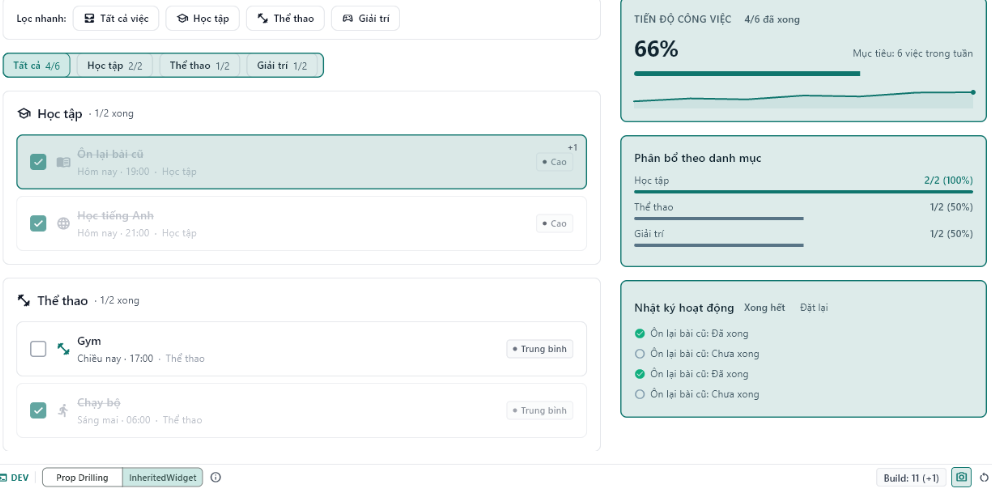
\includegraphics[width=0.96\linewidth, height=4.30cm, keepaspectratio]{figures/demo_taskflow_tight.png}%
  }

  \vspace{0.12cm}
  \begin{tcolorbox}[
    enhanced,
    colback=CodeBg,
    colframe=DarkMain,
    arc=2.5pt,
    left=8pt, right=8pt, top=4.0pt, bottom=4.0pt
  ]
    \fontsize{8.5pt}{11.5pt}\selectfont
    \textbf{Nhìn vào đâu}: Bấm hoàn thành việc ở \textbf{Danh sách việc} (trái) $\to$ \textbf{Tiến độ} (phải) tự động cập nhật.
  \end{tcolorbox}
\end{frame}

% ==============================================================================
% Slide 14: Trường hợp 1: Kỹ thuật Prop Drilling
% ==============================================================================
\begin{frame}[fragile]{Trường hợp 1: Kỹ thuật Prop Drilling}
  \vspace{-0.15cm}
  \begin{columns}[c, onlytextwidth]
    \begin{column}{0.43\textwidth}
      \begin{codepanel}[top=8pt, bottom=8pt]
\begin{Verbatim}[commandchars=§«»,fontsize=\fontsize{7.2pt}{10.2pt}\selectfont]
§cmt«// Gọi setState() ở gốc HomeScreen:»
void _handleToggleTask(String id) {
  §hl«setState(() {»
    _model.toggleTask(id);
  §hl«});» §cmt«// Toàn bộ cây con build lại!»
}
\end{Verbatim}
      \end{codepanel}

      \vspace{0.22cm}
      \begin{tcolorbox}[
        enhanced,
        colback=DarkMain!8,
        colframe=DarkMain,
        arc=3pt,
        left=8pt, right=8pt, top=6pt, bottom=6pt
      ]
        {\large\bfseries\color{DarkMain} Build lan truyền: \textbf{+14}}\\[0.08cm]
        {\small Toàn bộ màn hình, nhóm danh mục và 6 thẻ đều bị build lại thừa.}
      \end{tcolorbox}
    \end{column}%
    \hfill%
    \begin{column}{0.55\textwidth}
      \centering
      \setlength{\fboxsep}{0pt}\fcolorbox{DarkMain}{white}{%
        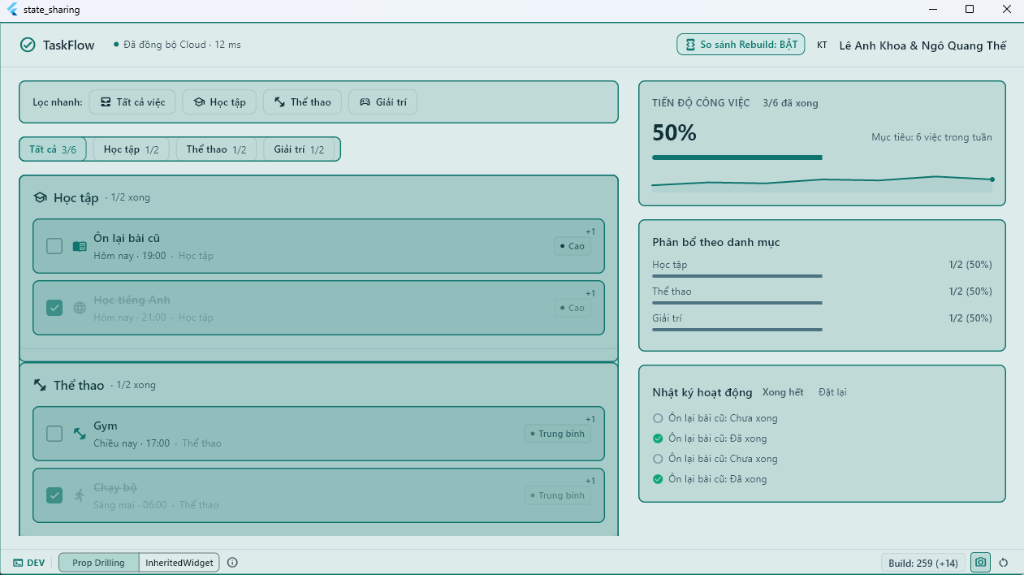
\includegraphics[width=\dimexpr\linewidth-1.6pt\relax, height=4.80cm, keepaspectratio]{figures/taskflow_prop_drilling.png}%
      }
    \end{column}%
  \end{columns}
\end{frame}

% ==============================================================================
% Slide 15: Luồng trạng thái trong ứng dụng TaskFlow
% ==============================================================================
\begin{frame}[fragile]{Luồng trạng thái trong ứng dụng TaskFlow}
  \vspace{-0.15cm}
  \centering
  \begin{tikzpicture}
    \node[subbox, text width=1.90cm, align=center, minimum height=0.85cm, inner sep=2.5pt] (c1) at (-5.45, 0)
      {\textbf{\small Tương tác}\\[1pt]{\scriptsize Checkbox / Lọc}};
    \node[diagbox, text width=2.45cm, align=center, minimum height=0.85cm, inner sep=2.5pt] (c2) at (-1.80, 0)
      {{\fontsize{8.5pt}{9.8pt}\selectfont\textbf{TaskFlowModel}}\\[1pt]{\scriptsize Xử lý logic}};
    \node[subbox, text width=1.80cm, align=center, minimum height=0.85cm, inner sep=2.5pt] (c3) at (1.80, 0)
      {\textbf{\small Notifier}\\[1pt]{\scriptsize Phát tín hiệu}};
    \node[diagbox, text width=2.60cm, align=center, minimum height=0.85cm, inner sep=3.0pt] (c4) at (5.45, 0)
      {\textbf{\small Widget con}\\[1pt]{\scriptsize Build lại cục bộ}};

    \draw[flowarrow] (c1.east) -- (c2.west) node[midway, above=4.0pt, font=\fontsize{7.8pt}{9pt}\selectfont\bfseries\color{DarkMain}] {invoke};
    \draw[flowarrow] (c2.east) -- (c3.west) node[midway, above=4.0pt, font=\fontsize{7.8pt}{9pt}\selectfont\bfseries\color{DarkMain}] {notify};
    \draw[flowarrow] (c3.east) -- (c4.west) node[midway, above=4.0pt, font=\fontsize{7.8pt}{9pt}\selectfont\bfseries\color{DarkMain}] {update};
  \end{tikzpicture}

  \vspace{0.18cm}
  \begin{columns}[T, onlytextwidth]
    \begin{column}{0.50\textwidth}
      \fontsize{8.8pt}{13.2pt}\selectfont
      $\bullet$ \textbf{Khi người dùng tương tác}: Checkbox hoặc bộ lọc gọi hàm trên \code{TaskFlowModel} để cập nhật dữ liệu.\\[0.22cm]
      $\bullet$ \textbf{Khi dữ liệu đổi}: Model gọi \code{notifyListeners()}, chỉ những widget đang đăng ký nghe mới build lại.
    \end{column}
    \hfill
    \begin{column}{0.46\textwidth}
      \begin{codepanel}[top=6pt, bottom=6pt]
\begin{Verbatim}[commandchars=§«»,fontsize=\fontsize{7.2pt}{10.0pt}\selectfont]
void toggleTask(String id) {
  _tasks[i] = _tasks[i].copyWith(...);
  §hl«notifyListeners();» §cmt«// Báo cho UI»
}
\end{Verbatim}
      \end{codepanel}
    \end{column}
  \end{columns}
\end{frame}

% ==============================================================================
% Slide 16: Trường hợp 2: InheritedWidget kết hợp Model
% ==============================================================================
\begin{frame}[fragile]{Trường hợp 2: InheritedWidget kết hợp Model}
  \vspace{-0.15cm}
  \begin{columns}[c, onlytextwidth]
    \begin{column}{0.43\textwidth}
      \begin{codepanel}[top=8pt, bottom=8pt]
\begin{Verbatim}[commandchars=§«»,fontsize=\fontsize{7.2pt}{10.2pt}\selectfont]
§cmt«// Thẻ lá tự đọc dữ liệu từ Scope O(1):»
Widget build(BuildContext context) {
  §hl«final scope = TaskScope.of(context);»
  final task = scope.tasks
      .firstWhere((t) => t.id == widget.id);
  return _buildTile(task);
}
\end{Verbatim}
      \end{codepanel}

      \vspace{0.22cm}
      \begin{tcolorbox}[
        enhanced,
        colback=DarkMain!8,
        colframe=DarkMain,
        arc=3pt,
        left=8pt, right=8pt, top=6pt, bottom=6pt
      ]
        {\large\bfseries\color{DarkMain} Build cục bộ: \textbf{+1}}\\[0.08cm]
        {\small Chỉ duy nhất thẻ được click build lại, các widget khác không bị ảnh hưởng.}
      \end{tcolorbox}
    \end{column}%
    \hfill%
    \begin{column}{0.55\textwidth}
      \centering
      \setlength{\fboxsep}{0pt}\fcolorbox{DarkMain}{white}{%
        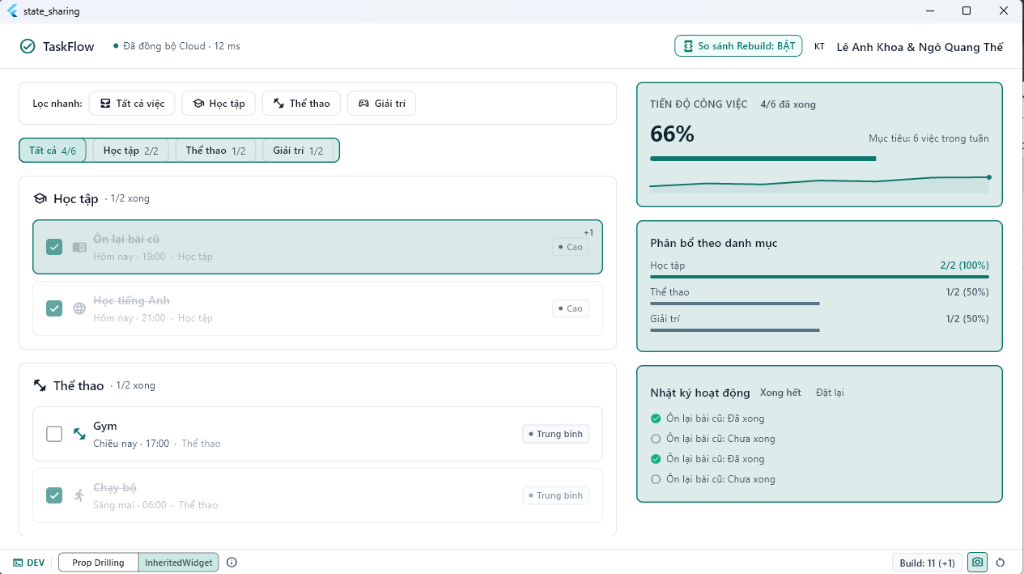
\includegraphics[width=\dimexpr\linewidth-1.6pt\relax, height=4.80cm, keepaspectratio]{figures/taskflow_inherited_widget.png}%
      }
    \end{column}%
  \end{columns}
\end{frame}

% ==============================================================================
% Slide 17: Kết quả đo lường và đánh giá thực nghiệm
% ==============================================================================
\begin{frame}{Kết quả đo lường và đánh giá thực nghiệm}
  \vspace{-0.22cm}
  % Hàng 3 số liệu lớn nổi bật
  \begin{columns}[c, onlytextwidth]
    \begin{column}{0.31\textwidth}
      \begin{tcolorbox}[enhanced, colback=DarkMain!10, colframe=DarkMain, arc=3pt, halign=center, top=5pt, bottom=5pt]
        {\Huge\bfseries\color{DarkMain} 14 $\to$ 1}\\[2pt]
        {\footnotesize\bfseries Lượt build khi tick việc}
      \end{tcolorbox}
    \end{column}
    \hfill
    \begin{column}{0.31\textwidth}
      \begin{tcolorbox}[enhanced, colback=DarkMain!10, colframe=DarkMain, arc=3pt, halign=center, top=5pt, bottom=5pt]
        {\Huge\bfseries\color{DarkMain} -92,9\%}\\[2pt]
        {\footnotesize\bfseries Giảm build thừa (khi tick 1 việc)}
      \end{tcolorbox}
    \end{column}
    \hfill
    \begin{column}{0.31\textwidth}
      \begin{tcolorbox}[enhanced, colback=DarkMain!10, colframe=DarkMain, arc=3pt, halign=center, top=5pt, bottom=5pt]
        {\Huge\bfseries\color{DarkMain} 2 $\to$ 0}\\[2pt]
        {\footnotesize\bfseries Widget trung gian}
      \end{tcolorbox}
    \end{column}
  \end{columns}

  \vspace{0.10cm}
  % Bảng đối chiếu 3 dòng đặt bên dưới
  \renewcommand{\arraystretch}{1.12}
  \setlength{\tabcolsep}{6.0pt}
  \fontsize{8.2pt}{11.0pt}\selectfont
  \centering
  \begin{tabular}{@{} l c c r @{}}
    \toprule[0.9pt]
    \textbf{Thao tác thử nghiệm} & \textbf{Trường hợp 1} & \textbf{Trường hợp 2} & \textbf{Hiệu quả cải thiện} \\
    & {\scriptsize\color{TextMuted}(Prop Drilling)} & {\scriptsize\color{TextMuted}(InheritedWidget)} & \\
    \midrule[0.5pt]
    Tick 1 công việc & 14 & 1 & \textbf{Giảm 92,9\%} build thừa \\
    Lọc nhanh danh mục & 14 & 4 & \textbf{Giảm 71,4\%} build thừa \\
    Xong tất cả / Đặt lại & 14 & 8 & \textbf{Giảm 42,9\%} build thừa \\
    \bottomrule[0.9pt]
  \end{tabular}

  \vspace{0.10cm}
  {\small\color{TextMuted} \textbf{Kết luận}: Trường hợp \textbf{InheritedWidget kết hợp Model} giúp giảm 42,9--92,9\% lượt build thừa so với Trường hợp 1.}
\end{frame}

% ==============================================================================
% Slide 18: Cập nhật cục bộ từng thẻ với ValueNotifier
% ==============================================================================
\begin{frame}[fragile]{Cập nhật cục bộ từng thẻ với ValueNotifier}
  \vspace{-0.15cm}
  \begin{columns}[c, onlytextwidth]
    \begin{column}{0.48\textwidth}
      \begin{codepanel}[top=8pt, bottom=8pt]
\begin{Verbatim}[commandchars=§«»,fontsize=\fontsize{7.2pt}{10.2pt}\selectfont]
§cmt«// Tách Notifier riêng cho từng ID:»
void toggleTask(String id) {
  §hl«_taskNotifiers[id]?.value = updated;»
}

§cmt«// Bọc Builder tại cấp lá:»
ValueListenableBuilder<TaskItem>(
  valueListenable: model.getNotifier(id),
  builder: (context, item, _) => TaskTile(item),
);
\end{Verbatim}
      \end{codepanel}
    \end{column}
    \hfill
    \begin{column}{0.48\textwidth}
      \begin{codepanel}[top=10pt, bottom=10pt]
        {\small\bfseries\color{DarkMain} Hướng cải tiến: Tách Notifier cho từng thẻ}\\[0.20cm]
        \fontsize{8.8pt}{13.5pt}\selectfont
        $\bullet$ \textbf{Cơ chế}: Gán cho mỗi thẻ công việc một \code{ValueNotifier} riêng biệt thay vì dùng chung cả Model.\\[0.22cm]
        $\bullet$ \textbf{Hiệu quả}: Khi tick một việc, chỉ build lại đúng thẻ có thay đổi thông qua \code{ValueListenableBuilder}.
      \end{codepanel}
    \end{column}
  \end{columns}
\end{frame}

% ==============================================================================
% Slide 19: Kết luận: Khi nào dùng cơ chế nào
% ==============================================================================
\setsectionfooter{Tổng kết}
\begin{frame}{Kết luận: Khi nào dùng cơ chế nào}
  \vspace{0.20cm}
  \renewcommand{\arraystretch}{1.40}
  \setlength{\tabcolsep}{8.0pt}
  \fontsize{9.0pt}{12.5pt}\selectfont
  \centering
  \begin{tabular}{@{} >{\bfseries\color{DarkMain}}l >{\raggedright\arraybackslash}p{4.6cm} >{\raggedright\arraybackslash}p{4.6cm} @{}}
    \toprule[0.9pt]
    \textbf{Cơ chế} & \textbf{Dùng khi} & \textbf{Đặc điểm} \\
    \midrule[0.5pt]
    Constructor / Callback & Cha--con 1--2 tầng & Đơn giản, không thêm class phụ \\
    \addlinespace[0.18cm]
    InheritedWidget & Toàn cây, state dùng chung & Tra cứu trực tiếp $O(1)$, Theme, Config \\
    \addlinespace[0.18cm]
    Change / ValueNotifier & Dữ liệu hay thay đổi, có logic & Chỉ build lại widget lắng nghe \\
    \bottomrule[0.9pt]
  \end{tabular}

  \vspace{0.50cm}
  \begin{center}
    {\small\color{TextMuted} \textbf{Nên nhớ}: Bắt đầu từ cách đơn giản nhất, chỉ dùng Notifier hoặc InheritedWidget khi cần truyền qua nhiều tầng.}
  \end{center}
\end{frame}

% ==============================================================================
% Slide 20: Tài liệu tham khảo
% ==============================================================================
\setsectionfooter{Tài liệu tham khảo}
\begin{frame}{Tài liệu tham khảo}
  \vspace{0.02cm}
  \begin{enumerate}\setlength{\itemsep}{0.08cm}
    \footnotesize
    \item Flutter Documentation, \textit{``Differentiate between ephemeral state and app state''}, Google.\\
          {\color{DarkMain}\url{https://docs.flutter.dev/data-and-backend/state-mgmt/ephemeral-vs-app}}
    \item Flutter Documentation, \textit{``InheritedWidget class''}, Google.\\
          {\color{DarkMain}\url{https://api.flutter.dev/flutter/widgets/InheritedWidget-class.html}}
    \item Flutter Documentation, \textit{``ListenableBuilder class''}, Google.\\
          {\color{DarkMain}\url{https://api.flutter.dev/flutter/widgets/ListenableBuilder-class.html}}
    \item Flutter Documentation, \textit{``ValueNotifier$<$T$>$ class''}, Google.\\
          {\color{DarkMain}\url{https://api.flutter.dev/flutter/foundation/ValueNotifier-class.html}}
    \item TS. Nguyễn Duy Nhật Viễn, \textit{``Bài giảng Lập trình Đa nền tảng''}, Khoa Điện tử và Trí tuệ Nhân tạo, Trường Đại học Bách khoa --- Đại học Đà Nẵng, 2026.
  \end{enumerate}

  \vspace{0.18cm}
  \begin{codepanel}
    {\bfseries\color{DarkMain} Mã nguồn chương trình thực nghiệm trên GitHub}\\[2pt]
    {\footnotesize\ttfamily\color{DarkMain} https://github.com/KhoaLe246205/cross-platform/tree/main/state\_sharing}
  \end{codepanel}
\end{frame}

% ==============================================================================
% Slide 21: Cảm ơn
% ==============================================================================
\setsectionfooter{}
\begin{frame}
  \vspace{1.95cm}
  \centering
  {\fontsize{19.5pt}{25pt}\selectfont\bfseries\color{DarkMain}
    Cảm ơn Thầy và các bạn đã lắng nghe!\par
  }
\end{frame}

\end{document}
